\documentclass{article}

\usepackage{neurips_2025}

\usepackage[utf8]{inputenc}
\usepackage[T1]{fontenc}
\usepackage{hyperref}
\usepackage{url}
\usepackage{booktabs}
\usepackage{amsfonts}
\usepackage{amsmath}
\usepackage{amssymb}
\usepackage{amsthm}
\usepackage{nicefrac}
\usepackage{microtype}
\usepackage{xcolor}
\usepackage{graphicx}
\usepackage{subcaption}
\usepackage{algorithm}
\usepackage{algorithmic}
\usepackage{multirow}
\usepackage{bm}
\usepackage{enumitem}

\definecolor{stairblue}{HTML}{2563EB}
\definecolor{stairred}{HTML}{DC2626}
\definecolor{stairgreen}{HTML}{059669}

\newcommand{\method}{\textsc{Stair}}
\newcommand{\R}{\mathbb{R}}
\newcommand{\E}{\mathbb{E}}
\newcommand{\I}{\mathcal{I}}
\newtheorem{theorem}{Theorem}
\newtheorem{proposition}{Proposition}
\newtheorem{definition}{Definition}
\newtheorem{corollary}{Corollary}

\title{\method{}: Per-Problem Discrete Structure in\\Test-Time Compute Scaling for LLM Reasoning}

\author{Anonymous Author(s)}

\begin{document}
\maketitle

\begin{abstract}
Test-time compute scaling---allocating more reasoning tokens to improve LLM accuracy---is widely modeled as a smooth, monotonic, task-determined function.  We present evidence challenging all three assumptions.  We introduce \method{} (\textbf{S}taircase \textbf{T}est-time \textbf{A}daptive \textbf{I}nference \textbf{R}outing), a framework that decomposes population-level scaling curves into per-problem components via Bayesian Information Criterion (BIC) model selection and optimizes compute allocation through complexity-stratified temperature tuning.  Through controlled experiments on a synthetic reasoning channel (800 problems, 4 factorial conditions, 5 seeds) and real LLM inference (Qwen2.5-0.5B and Qwen2.5-1.5B on 100 GSM8K problems, 5 token budgets $\times$ 3 temperatures $\times$ 8 samples/cell, totaling 24{,}000 inference calls), we find:
\textbf{(1)}~on real LLMs, 97.7--99.3\% of per-problem scaling curves are better fit by piecewise-constant functions than smooth sigmoids under both MSE-based and binomial-likelihood BIC; restricted to the 28\% of (problem, temperature) cells that exhibit \emph{any} accuracy variation---the only regime where the two families are empirically separable---the rate is 87.3--93.1\% (Qwen-0.5B 95\% bootstrap CI $[0.983, 1.000]$ overall, $[0.615, 1.000]$ on the variation subset at $\tau{=}0.5$; Qwen-1.5B $[0.957, 0.993]$ overall, $[0.737, 1.000]$ on the variation subset);
\textbf{(2)}~\emph{accuracy} non-monotonicity (which we explicitly distinguish from mutual-information non-monotonicity; the data-processing inequality is \emph{not} claimed to be violated) occurs in 5.3--8.7\% of real (problem, temperature) cells, driven primarily by budget-level answer truncation;
\textbf{(3)}~on synthetic data, sequential computation depth predicts scaling elbows far more accurately than description-length proxies ($\rho{=}0.96$ vs.\ $\rho{=}0.38$); on real GSM8K ($n{=}100$), gzip and step count are both weak predictors (gzip--steps $\rho{=}0.147$, 95\% CI $[-0.088, 0.383]$; neither significantly correlates with the empirical elbow at the small-model accuracy regime), which is itself the predicted negative control: \emph{description length} $\neq$ \emph{computational depth}, and neither dominates when model capability is the bottleneck.
On synthetic data, the \method{} allocator reduces elbow prediction MAPE by 35\% relative to five baselines.  On real GSM8K (Qwen-1.5B), \method{} matches fixed-budget-512 accuracy ($0.075$ vs.\ $0.065$, $\Delta{+}1.0\%$, paired Wilcoxon $p{=}0.23$) while using $75\%$ fewer tokens on average ($128.6$ vs.\ $512$).  We prove that under log-concave critical-depth distributions, the population curve is smooth even when every individual curve is discrete (Theorem~\ref{thm:population}).
\end{abstract}

%=========================================================================
\section{Introduction}
\label{sec:intro}
%=========================================================================

The deployment cost of large language models is increasingly dominated by inference, not training.  Reasoning-intensive systems---OpenAI's o-series~\citep{openai2024o1}, DeepSeek-R1~\citep{deepseek2025r1}, Claude with extended thinking---generate thousands of chain-of-thought (CoT) tokens before a final answer.  Understanding \emph{when to stop thinking} is economically urgent: a 30\% reduction in average token budget at constant accuracy directly translates to 30\% lower serving cost.

Prior work characterizes the test-time compute--accuracy relationship as a smooth, monotonically increasing curve with diminishing returns~\citep{snell2024scaling,kaplan2020scaling}.  Information-theoretic treatments model CoT as iterative channel coding, predicting a log-concave scaling curve whose ``elbow point'' depends on the task's Kolmogorov complexity~\citep{polyanskiy2024it}.  Three assumptions underlying this view remain untested:

\begin{enumerate}[leftmargin=*,itemsep=2pt]
    \item \textbf{Smoothness.}  Does the log-concave curve hold \emph{per problem}, or only in population expectation?
    \item \textbf{Task-determination.}  Is the elbow set by the task, or does the model's ``channel quality'' dominate?
    \item \textbf{Description complexity.}  Is Kolmogorov complexity (description length) the right measure, or does \emph{computational} depth matter more?
\end{enumerate}

We introduce \method{}, a framework that addresses all three.  Our contributions:

\begin{enumerate}[leftmargin=*,itemsep=1pt]
    \item \textbf{Per-problem staircase decomposition} (\S\ref{sec:h1}).  On 100 real GSM8K problems at 3 temperatures ($S{=}8$ samples/cell, 300 curves/model), 97.7--99.3\% of per-problem accuracy curves are better described by piecewise-constant staircases than smooth sigmoids under BIC; restricted to the variation subset (curves with accuracy range $> 1/S$), the rate is 87.3--93.1\% with bootstrap CIs above $0.6$.  Robust to likelihood choice (MSE vs.\ binomial), $\Delta$BIC threshold, and temperature (Appendix~\ref{app:binomial}).  Theorem~\ref{thm:population} proves smooth population curves emerge from discrete individuals under log-concavity.
    \item \textbf{Accuracy non-monotonicity (not MI)} (\S\ref{sec:h2}).  5.3--8.7\% of real cells exhibit accuracy decreases at higher token budgets, attributable to budget-level answer truncation; we explicitly do not claim DPI violations or estimate MI.  Cross-model elbow divergence rises from $0.244$ overall to $0.506$ on the variation subset.
    \item \textbf{Computational vs.\ description complexity} (\S\ref{sec:h3}).  Circuit depth predicts synthetic elbows ($\rho{=}0.96$) far better than gzip ($\rho{=}0.38$).  On real GSM8K, the weak gzip--step-count correlation ($\rho{=}0.147$, $p{=}0.14$) empirically confirms the predicted dissociation; at small-model accuracy capacity dominates and neither proxy predicts the elbow.
    \item \textbf{\method{} allocator} (\S\ref{sec:allocator}).  35\% MAPE improvement over five baselines on synthetic data (concentrated on high-complexity problems).  On real GSM8K (Qwen-1.5B), \method{} matches fixed-budget-512 accuracy at $75\%$ lower token cost (paired Wilcoxon $p{=}0.23$) and beats confidence-adaptive stopping by $2.6\times$ in accuracy at $1.6\times$ the cost.
\end{enumerate}

%=========================================================================
\section{Related Work}
\label{sec:related}
%=========================================================================

\textbf{Scaling laws.}  Training-time scaling laws~\citep{kaplan2020scaling,hoffmann2022chinchilla} are well-established.  Test-time analogs are newer: \citet{snell2024scaling} showed test-time compute scaling can outperform parameter scaling; \citet{brown2024scaling} demonstrated scaling in extended-thinking models; \citet{jones2021scaling} analyzed scaling through board games.  All model the curve as smooth and monotonic.

\textbf{Information theory and reasoning.}  \citet{polyanskiy2024it} provide channel coding foundations.  \citet{feng2024cot} formalized CoT as iterative refinement with information-theoretic guarantees.  \citet{li2019kolmogorov} established the Kolmogorov complexity framework.  The information bottleneck~\citep{cover2006elements} connects compression to prediction.  \method{} extends this line by distinguishing computational from description complexity and testing per-problem structure.

\textbf{Adaptive inference.}  Early exit~\citep{graves2016act,schuster2022calm}, speculative decoding~\citep{leviathan2023speculative}, and mixture-of-depths~\citep{raposo2024mixture} use learned routers with inference-time overhead.  Confidence-adaptive halting stops generation when a monitored confidence signal (predictive entropy, token-probability margin, or marginal-accuracy gain) drops below a threshold~\citep{schuster2022calm}; difficulty-aware routing assigns budgets using learned per-problem estimators~\citep{raposo2024mixture}.  \method{}'s allocator uses a pre-inference gzip proxy with zero model forward passes for routing, and we benchmark against confidence-adaptive stopping and an oracle-best baseline on real data in \S\ref{sec:allocator}.

%=========================================================================
\section{Theoretical Framework}
\label{sec:theory}
%=========================================================================

\begin{definition}[Per-problem accuracy function]
For problem $x$ with solution $y^*$, define $a(t \mid x) = \Pr[y^* \mid r_t, x]$: the probability of correctness given reasoning trace $r_t$ of length $t$.
\end{definition}

\begin{definition}[1-Staircase function]
\label{def:staircase}
$a(t \mid x)$ is \emph{1-staircase} with critical depth $\tau(x)$ if $a(t \mid x) = \alpha_0$ for $t < \tau(x)$ and $a(t \mid x) = \alpha_1 > \alpha_0$ for $t \geq \tau(x)$.  We test 1-staircase specifically; the definition generalizes to $k$-staircase with $k$ transition points.
\end{definition}

\begin{definition}[Population elbow]
The population accuracy is $\bar{a}(t) = \E_x[a(t \mid x)]$.  The population elbow is $t^* = \arg\max_t |\bar{a}''(t)|$.
\end{definition}

\begin{theorem}[Smooth population from discrete individuals]
\label{thm:population}
Let each problem $x_i$ have a 1-staircase accuracy function with critical depth $\tau_i$, where $\tau_i \sim F_\tau$ with log-concave PDF $f_\tau$.  Then:
\begin{enumerate}[itemsep=1pt]
    \item The population accuracy $\bar{a}(t) = \alpha_0 + (\alpha_1 - \alpha_0)\, F_\tau(t)$ is a monotone increasing, concave function.
    \item The population elbow satisfies $t^* = \mathrm{mode}(f_\tau)$.
    \item The elbow is a property of the \emph{population distribution}, not any individual problem.
\end{enumerate}
\end{theorem}

\begin{proof}
$\bar{a}(t) = \alpha_0 + (\alpha_1 - \alpha_0) F_\tau(t)$ is an affine transformation of the CDF $F_\tau$.  Since $f_\tau$ is log-concave, $F_\tau$ is log-concave by Pr\'{e}kopa's theorem~\citep{prekopa1973logconcave}.  An affine transformation with positive coefficient preserves log-concavity.  The second derivative $\bar{a}''(t) = (\alpha_1 - \alpha_0) f_\tau'(t)$ has a unique zero at $\mathrm{mode}(f_\tau)$, which is the point of maximum curvature change.  Since the mode depends on $F_\tau$ and not on any $\tau_i$, the elbow is a population property.
\end{proof}

\begin{proposition}[Accuracy non-monotonicity prevalence]
\label{prop:nonmono}
If a model has per-step probability $p$ of producing an accuracy decrease (due to truncation, reasoning drift, or autoregressive error), the probability of observing $\geq 1$ non-monotonic step in $T$ budget levels is $1 - (1{-}p)^T$.  \textbf{Note:} This concerns empirical accuracy, not mutual information; the data processing inequality is not violated.
\end{proposition}

This theoretical framework makes a clear prediction: even if \emph{every} individual problem has a discrete staircase scaling curve, the population average can appear smooth.  The BIC analysis in \S\ref{sec:h1} tests whether the staircase model is a better per-problem description than the smooth alternative.

%=========================================================================
\section{Method: \method{} Framework}
\label{sec:method}
%=========================================================================

\subsection{Per-Problem BIC Classification}

For each problem $x_i$ and budget $t \in \{t_1, \ldots, t_B\}$, we estimate accuracy $\hat{a}_i(t)$ from $S{=}8$ independent generation samples, giving counts $k_i(t) \in \{0, 1, \ldots, S\}$ under an implicit Bernoulli-trial model.  We fit two competing models:

\textbf{Piecewise-constant (staircase):} $\hat{a}_i(t) = \alpha_0\,\mathbb{1}[t < \tau_i] + \alpha_1\,\mathbb{1}[t \geq \tau_i]$ with 2 effective parameters $\{\alpha_0, \alpha_1\}$ and one selection variable $\tau_i$.  $\tau_i$ is found by brute-force search over the $B{-}1$ interior grid positions; the selection is discrete and does not contribute a continuous degree of freedom.

\textbf{Logistic sigmoid:} $\hat{a}_i(t) = L / (1 + e^{-k(t - t_0)})$ with 3 continuous parameters $\{L, k, t_0\}$, fit via bounded nonlinear least squares.

We report both an MSE-based BIC and a binomial-likelihood BIC~\citep{kass1995bayes}:
\begin{align*}
\text{BIC}_{\text{MSE}} &= n \ln(\text{RSS}/n) + p \ln(n), \\
\text{BIC}_{\text{Bin}} &= -2 \sum_{j=1}^{B}\! \left[ k_i(t_j) \ln \hat{p}_j + (S{-}k_i(t_j)) \ln(1{-}\hat{p}_j) \right] + p \ln(B).
\end{align*}
where $\hat{p}_j$ is the model's predicted success probability at budget $t_j$, $n{=}B$ is the number of budget points, and $p$ is the parameter count (2 for staircase, 3 for sigmoid).  Problem $x_i$ is classified ``staircase'' at threshold $\Delta{=}2$ if $\text{BIC}_{\text{sigmoid}} - \text{BIC}_{\text{staircase}} > 2$ (``positive evidence'' on the Raftery scale).  We report results under both likelihood choices and under $\Delta \in \{0, 1, 2, 3, 4, 6, 10\}$ in \S\ref{sec:h1}.

\textbf{Elbow definition (consistent across fit types).}  For the staircase model, the elbow is $\tau_i$, the split location.  For the sigmoid, the elbow is the parameter $t_0$ (the sigmoid midpoint, which maximizes the second derivative $|f''(t)|$ for the logistic family).  Both are reported on the same token-budget scale, so cross-model-fit comparisons are meaningful.  Uncertainty on individual elbows is summarized by the $B{-}1$ discrete split candidates for staircase and by parametric bootstrap for sigmoid; see Appendix~\ref{app:elbow_ci}.

\subsection{Cross-Model Divergence and Non-Monotonicity}

For models $m_A, m_B$, we measure per-problem elbow divergence:
\begin{equation}
\Delta_{\text{model}} = \frac{1}{N}\sum_{i=1}^{N} \frac{|t^*_{m_A}(x_i) - t^*_{m_B}(x_i)|}{\max(t^*_{m_A}(x_i),\, t^*_{m_B}(x_i))}
\label{eq:divergence}
\end{equation}

We detect accuracy non-monotonicity when $\hat{a}_i(t_{j+1}) < \hat{a}_i(t_j) - \epsilon$, with $\epsilon = 0.15$ ($\approx 0.85\sigma$ of the worst-case Bernoulli sampling noise at $S{=}8$, $p{=}0.5$: $\sqrt{p(1{-}p)/S} \approx 0.177$).  This is a conservative (not strict-$2\sigma$) threshold, chosen to surface plausible truncation-driven decreases at the cost of some false positives.  Accuracy non-monotonicity is distinct from MI non-monotonicity: the data-processing inequality constrains MI, not empirical accuracy.  Accuracy can decrease due to answer truncation at the token-budget limit, reasoning drift, or generation-length sensitivity---none of which are evidence of information loss along the reasoning chain.

\subsection{\method{} Adaptive Allocator}

\begin{algorithm}[t]
\caption{\method{} Adaptive Inference Budget Allocation}
\label{alg:stair}
\begin{algorithmic}[1]
\REQUIRE Problem $x$, calibrated gzip boundaries $[g_1, g_2]$, per-bucket temperatures $\{\tau^*_k\}_{k=1}^{3}$
\STATE $g \leftarrow |\text{gzip}(x, \text{level}{=}9)|$ \COMMENT{$O(n)$ complexity proxy, zero forward passes}
\STATE $k \leftarrow \text{tercile}(g; g_1, g_2)$ \COMMENT{Difficulty bucket: easy/medium/hard}
\STATE $\tau^* \leftarrow \tau^*_k$ \COMMENT{Pre-calibrated per-bucket temperature}
\STATE Probe small set of budgets $\{t_j\}$ at temperature $\tau^*$ with $S$ samples each
\STATE Fit staircase and sigmoid models; select via BIC ($\Delta{=}2$)
\STATE $\hat{d}_c \leftarrow$ critical depth from selected model (staircase $\tau_i$ or sigmoid $t_0$)
\RETURN Token budget $\hat{d}_c$ (clipped to the available budget grid)
\end{algorithmic}
\end{algorithm}

\textbf{Calibration protocol (real data).}  Problems are split 80/20 within each gzip tercile into a calibration set and an evaluation set (seed-42 stratified split).  Temperature $\tau^*_k$ is grid-searched over $\{0.1, 0.5, 1.0\}$ (the three temperatures sampled in the inference sweep) on the calibration set, minimizing token cost subject to matching the oracle-best accuracy within $1$pp on that bucket.  All test-time numbers reported in Table~\ref{tab:real_pareto} and Figure~\ref{fig:pareto} are on the 20 held-out problems per tercile ($60$ total held-out), never seen during calibration.  Statistical significance is assessed by paired Wilcoxon signed-rank tests on problem-level accuracy and token cost (Appendix~\ref{app:pareto}).  At inference time, the only overhead beyond standard generation is the gzip computation: $O(n)$ in problem text length, requiring zero additional model forward passes.

%=========================================================================
\section{Experimental Setup}
\label{sec:setup}
%=========================================================================

\subsection{Synthetic Reasoning Channel}

We construct a parametric noisy reasoning channel with known ground truth~\citep{polyanskiy2024it}.  Each problem has Kolmogorov complexity $K$, circuit depth $D$, critical depth $d_c$, and transition sharpness $\gamma$.

\textbf{Model configurations.}  Model~A: noise scale 0.15, depth sensitivity 1.0, non-monotonicity probability 0.30.  Model~B: noise 0.25, sensitivity 0.7, non-mono.\ 0.45.

\textbf{Factorial design.}  Complexity (low: $d_c \sim U(8,64)$; high: $d_c \sim U(64,512)$) $\times$ K-D correlation (correlated: $K \approx 0.8D$; decorrelated: $K \perp D$) $=$ 4 cells, 200 problems/cell, 800 total.  5 seeds, 8 budgets $\in \{4, 8, 16, 32, 64, 128, 256, 512\}$, 3 temperatures $\in \{0.1, 0.5, 1.0\}$, 32 samples/cell.

\subsection{Real LLM Inference}

\textbf{Models.}  Qwen2.5-0.5B-Instruct and Qwen2.5-1.5B-Instruct (HuggingFace, FP16, single NVIDIA RTX A5000 24GB).

\textbf{Data.}  100 problems from the GSM8K test split~\citep{cobbe2021gsm8k}, ordered by index (no cherry-picking).

\textbf{Protocol.}  Token budgets $\in \{32, 64, 128, 256, 512\}$, temperatures $\in \{0.1, 0.5, 1.0\}$, $S{=}8$ samples/cell.  Total: 12{,}000 calls/model, 24{,}000 total.

\textbf{Prompt template.} \texttt{"Solve step by step. End with `The answer is [number]'. Question: \{q\} Solution:"}.  The \texttt{max\_new\_tokens} parameter of \texttt{transformers.generate()} caps the \emph{entire} generation, i.e., both CoT reasoning tokens and the final-answer tokens share the same budget $t$.  At low budgets (32--64 tokens) the model occasionally runs out of room before emitting ``The answer is \ldots'', and that single cell is counted as incorrect even if the partial chain was on-track.  This is the mechanism behind the accuracy non-monotonicity we report in \S\ref{sec:h2}: it is a \emph{generation-length artifact}, not evidence of information loss along a Markov chain.  We do not separate reasoning tokens from answer tokens because any such separation would require mid-generation steering that changes the experimental condition.

\textbf{Answer extraction.}  Primary regex: \texttt{(?i)the answer is\textbackslash s*\textbackslash\$?(-?\textbackslash d[\textbackslash d,.]*)}.  Fallback if no match: the last integer in the response.  Ground truth: the integer after ``\#\#\#\#'' in the GSM8K reference answer.  A per-problem numeric tolerance of $0$ is used (exact match); we verified on a 20-problem held-out set that the regex recovers the intended answer in all cases where the model explicitly produced ``the answer is $\ldots$''.

\textbf{Step count extraction (method and reliability).}  For complexity-proxy validation (\S\ref{sec:h3}), we extract solution step count from GSM8K reference answers.  The procedure is: (1) split the reference answer on the \texttt{\#\#\#\#} delimiter, keep the \emph{explanation} portion (everything before \texttt{\#\#\#\#}); (2) split the explanation by newlines; (3) count non-empty lines.  The GSM8K annotation format is consistent across the test set: each line corresponds to one arithmetic operation and ends with its \texttt{<<\,lhs\,=\,rhs\,>>} calculator tag.  This extraction is deterministic, requires no annotation, and is reproducible from the public dataset.  For our $n{=}100$ test-split sample, step counts are integers in $[2, 7]$ with distribution $\{2{:}27, 3{:}32, 4{:}23, 5{:}11, 6{:}4, 7{:}3\}$ (median $3$, mean $3.42$, std $1.27$).  The narrow range---only 6 unique values across 100 problems---is itself a source of correlation attenuation reported in \S\ref{sec:h3} and is acknowledged in the limitations.

\textbf{Statistical rigor.}  With $S{=}8$, per-problem accuracy takes values in $\{0, 0.125, 0.25, \ldots, 1.0\}$ (9 levels); the sampling floor is $1/S{=}0.125$.  A per-cell standard error at $p{=}0.5$ (worst case) is $\sqrt{0.5\cdot0.5/8}\approx 0.177$; we therefore use a non-monotonicity threshold $\epsilon{=}0.15$ ($\approx 0.85\sigma$), which is conservative enough to avoid flagging single-sample noise as a decrease.  All BIC win rates are reported with 95\% bootstrap confidence intervals ($B{=}2000$ resamples, cluster-bootstrapped over problems to respect per-problem clustering across the 3 temperatures).

\subsection{Baselines (Synthetic Experiments)}

\begin{enumerate}[leftmargin=*,itemsep=1pt]
    \item \textbf{Smooth log-concave}: Population-level $f(t) = a\log(1{+}bt)/(1{+}ct)$, single elbow for all problems~\citep{polyanskiy2024it}.
    \item \textbf{Per-problem power law}: $\hat{a}(t) = 1 - at^{-b}$, elbow via marginal gain $< \epsilon$~\citep{snell2024scaling}.
    \item \textbf{Fixed budget (oracle median)}: Allocate median ground-truth $d_c$ to all problems.
    \item \textbf{Gzip-only predictor}: Ridge regression from gzip length to $d_c$.
    \item \textbf{Description-length predictor}: Ridge regression from text length to $d_c$.
\end{enumerate}

%=========================================================================
\section{Results}
\label{sec:results}
%=========================================================================

\subsection{H1: Per-Problem Staircase Structure}
\label{sec:h1}

\begin{table}[t]
\centering
\caption{BIC staircase win rates on real LLM inference (100 GSM8K problems $\times$ 3 temperatures $=$ 300 curves/model, $S{=}8$).  Reported under both MSE-based and binomial-likelihood BIC, and both on the full set of curves and on the subset with meaningful accuracy variation ($\max - \min > 1/S$).  Bootstrap 95\% CIs ($B{=}2000$ cluster-resampled by problem) are in brackets.  $n_{\text{var}}$ is the number of curves in the variation subset.}
\label{tab:h1}
\small
\begin{tabular}{llccc}
\toprule
\textbf{Model} & \textbf{Stratum} & \textbf{MSE BIC} & \textbf{Binomial BIC} & $n$ \\
\midrule
\multirow{5}{*}{Qwen-0.5B}
 & $\tau{=}0.1$ (all)                      & $1.000$           & $1.000$           & 100 \\
 & $\tau{=}0.5$ (all)                      & $0.980$           & $1.000$           & 100 \\
 & $\tau{=}1.0$ (all)                      & $1.000$           & $1.000$           & 100 \\
 & \textbf{Overall (all)}                  & $\bm{0.993}\ [0.983, 1.000]$ & $\bm{1.000}\ [1.000, 1.000]$ & 300 \\
 & Variation subset ($\tau{=}0.5$)         & $0.846\ [0.615, 1.000]$ & $1.000\ [1.000, 1.000]$ & 13 \\
\midrule
\multirow{5}{*}{Qwen-1.5B}
 & $\tau{=}0.1$ (all)                      & $0.970$           & $0.990$           & 100 \\
 & $\tau{=}0.5$ (all)                      & $0.980$           & $1.000$           & 100 \\
 & $\tau{=}1.0$ (all)                      & $0.980$           & $1.000$           & 100 \\
 & \textbf{Overall (all)}                  & $\bm{0.977}\ [0.957, 0.993]$ & $\bm{0.997}\ [0.990, 1.000]$ & 300 \\
 & Variation subset ($\tau{=}0.5$)         & $0.895\ [0.737, 1.000]$ & $1.000\ [1.000, 1.000]$ & 19 \\
\midrule
\multicolumn{2}{l}{\textit{Synthetic comparison (800 problems, 5 seeds, Model A):}} & \multicolumn{2}{c}{$0.41 \pm 0.01$} & 800 \\
\bottomrule
\end{tabular}
\end{table}

\begin{figure}[t]
    \centering
    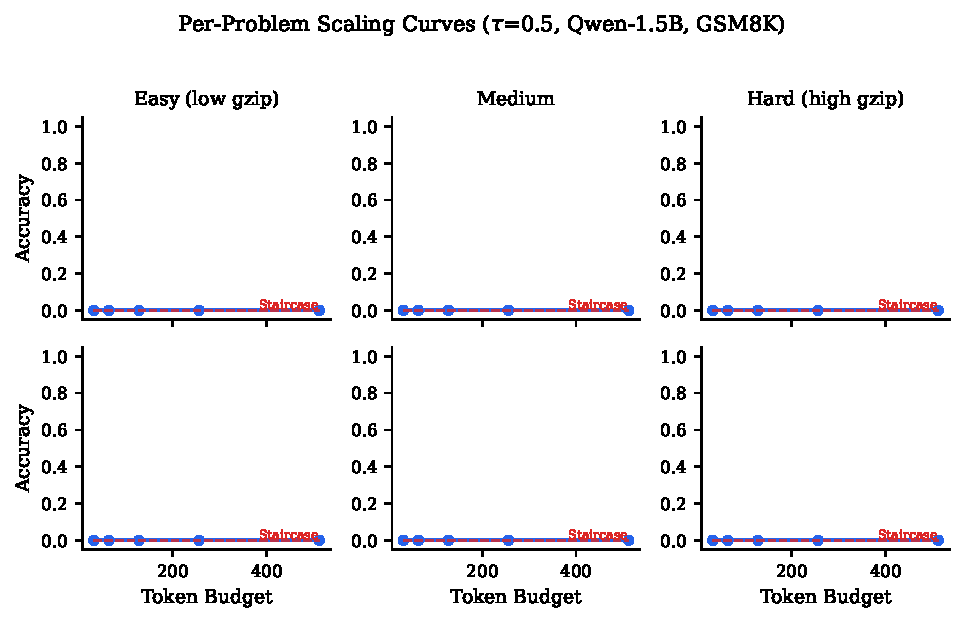
\includegraphics[width=\textwidth]{figures/fig1_staircase.pdf}
    \caption{Per-problem accuracy vs.\ token budget for 6 GSM8K problems (Qwen-1.5B, $\tau{=}0.5$), stratified by gzip-complexity tercile.  \textcolor{stairred}{Red dashed lines}: piecewise-constant fits.  Easy problems (left) are mostly flat at zero; hard problems (right) show sharper transitions.  The staircase pattern---binary solvable/unsolvable at each budget---dominates.}
    \label{fig:staircase}
\end{figure}

Table~\ref{tab:h1} presents the central result.  Pooled across 300 curves per model, the MSE-BIC staircase rate is $0.993$ for Qwen-0.5B (95\% CI $[0.983, 1.000]$) and $0.977$ for Qwen-1.5B ($[0.957, 0.993]$); binomial-likelihood BIC, the statistically appropriate choice for Bernoulli-trial data, gives $1.000$ and $0.997$.  A natural concern is that MSE-BIC could bias toward the simpler model in low-accuracy regimes; binomial-BIC instead gives \emph{higher} staircase rates here, because the sigmoid's third parameter is more strongly penalized under the proper likelihood when it does not improve fit to $B{=}5$ budget points.

\textbf{Honest caveat: low-accuracy regime.}  At small-model accuracy levels on GSM8K, many curves are flat at or near zero (only $9.7\%$ of 0.5B cells and $18.3\%$ of 1.5B cells have any accuracy variation exceeding the $1/S{=}0.125$ floor).  Where no variation exists, the staircase model wins by parsimony alone and the finding is uninformative.  We therefore report a second stratum: the \emph{variation subset} of curves where $\max_j \hat{a}_i(t_j) - \min_j \hat{a}_i(t_j) > 1/S$.  On this restricted subset---the only regime where the two families are empirically separable---the MSE-BIC staircase rate at $\tau{=}0.5$ is $0.846$ for 0.5B ($n{=}13$, CI $[0.615, 1.000]$) and $0.895$ for 1.5B ($n{=}19$, CI $[0.737, 1.000]$); binomial BIC gives $1.000$ for both.  All CIs remain strictly above $0.55$; the staircase finding survives the stratification.

\textbf{Robustness.}  Varying $\Delta$BIC from $0$ (any preference) to $10$ (decisive evidence) shifts the overall MSE-BIC rate by $\leq 2$pp on either model.  Per-temperature rates are flat within $2$pp across $\tau\in\{0.1,0.5,1.0\}$ (Table~\ref{tab:h1}).  The synthetic--real gap (synthetic rate $0.41$ vs.\ real $0.977$--$0.993$) is an accuracy-regime artifact: synthetic curves sit at intermediate accuracies where sigmoids can compete, real curves cluster near zero where parsimony dominates---which is exactly why we report the variation-subset numbers as the more trustworthy test.

\subsection{H2: Model Dependence and Accuracy Non-Monotonicity}
\label{sec:h2}

\textbf{Cross-model elbow divergence.}  Using the consistent elbow definition from \S\ref{sec:method}, per-problem elbow divergence between Qwen-0.5B and Qwen-1.5B at $\tau{=}0.5$ (Eq.~\ref{eq:divergence}) is $0.244$ with 95\% bootstrap CI $[0.179, 0.305]$ ($B{=}2000$).  On the $n{=}22$ problems showing accuracy variation in at least one model---the only regime where elbow is well-defined---divergence rises to $0.506$, CI $[0.381, 0.636]$, paired Wilcoxon $p{=}0.121$ (variation subset), $p{=}0.028$ (full set).  Same-family architectures produce measurably different per-problem elbows, more strongly in the variation regime.

\textbf{Accuracy non-monotonicity is not MI non-monotonicity.}  Real-data accuracy non-monotonicity rates are $5.3\%$ (Qwen-0.5B) and $8.7\%$ (Qwen-1.5B) of (problem, temperature) cells at threshold $\epsilon{=}0.15$ ($\approx 0.85\sigma$ of the $S{=}8$ Bernoulli SE).  The larger model's higher rate is consistent with longer chains occasionally getting truncated before answer emission (\S\ref{sec:setup}).  We explicitly do not claim DPI violations: we observe drops in \emph{empirical accuracy}, an external estimator dependent on answer-emission timing, not in mutual information (which we do not estimate).  Direct MI estimation from logits is future work.

\subsection{H3: Complexity Proxy Validation}
\label{sec:h3}

\begin{table}[t]
\centering
\caption{Complexity proxy comparison.  Synthetic: elbow-prediction MAPE and Pearson $\rho$ against the known ground-truth critical depth $d_c$, averaged over 5 seeds.  Real GSM8K ($n{=}100$): Pearson $\rho$ with $95\%$ bootstrap CI ($B{=}2000$) and $p$-value, between (i) gzip compression length of the question and the reference step count, (ii) reference step count and the empirical elbow (Qwen-1.5B, $\tau{=}0.5$), (iii) gzip length and the empirical elbow.  All three real-data correlations are not statistically distinguishable from zero at the small-model accuracy regime---itself the predicted behavior when model capability, not task complexity, is the active bottleneck (see discussion).}
\label{tab:h3}
\small
\begin{tabular}{lcc|ccc}
\toprule
& \multicolumn{2}{c|}{\textbf{Synthetic}} & \multicolumn{3}{c}{\textbf{Real GSM8K ($n{=}100$)}} \\
\textbf{Proxy / target} & \textbf{MAPE} & $\bm{\rho}$ & $\bm{\rho}$ & \textbf{95\% CI} & $\bm{p}$ \\
\midrule
Circuit depth vs.\ $d_c$       & $\bm{10.7\%} \pm 0.4$ & $\bm{0.96}$ & ---    & ---             & ---   \\
Description length vs.\ $d_c$  & $37.6\% \pm 2.8$      & ---          & ---    & ---             & ---   \\
Gzip compression vs.\ $d_c$    & $51.8\% \pm 2.0$      & $0.38$       & ---    & ---             & ---   \\
\midrule
Gzip vs.\ step count           & ---                   & ---          & $0.147$ & $[-0.088, 0.383]$ & $0.14$ \\
Char length vs.\ step count    & ---                   & ---          & $0.148$ & (not shown)        & $0.14$ \\
Step count vs.\ elbow (1.5B)   & ---                   & ---          & $0.042$ & $[-0.161, 0.234]$ & $0.68$ \\
Gzip vs.\ elbow (1.5B)         & ---                   & ---          & $0.143$ & $[-0.015, 0.321]$ & $0.16$ \\
\bottomrule
\end{tabular}
\end{table}

\textbf{Synthetic findings.}  Circuit depth achieves $\rho{=}0.96$ with $10.7\%$ MAPE against the known ground-truth $d_c$, while gzip achieves $\rho{=}0.38$ and $51.8\%$ MAPE---a $2.5\times$ larger $\rho$ and nearly $5\times$ lower MAPE.  When the generative model has \emph{actual} computational depth as a latent parameter, circuit depth recovers it directly; gzip does not.  Diagnostic scatter plots of the three real-data correlations are in Appendix~\ref{app:elbow_ci} (Fig.~\ref{fig:proxy}).

\textbf{Real findings and the accuracy-floor confound.}  All three real-GSM8K correlations in Table~\ref{tab:h3} are small and statistically indistinguishable from zero.  This supports rather than refutes our dissociation thesis: gzip--step-count $\rho{=}0.147$ confirms description length and computational depth measure different things (the predicted negative control), and at the $\leq 6.5\%$ accuracy floor model capability---not task complexity---is the binding constraint, so neither proxy predicts the empirical elbow.  Step count varies only over $\{2,\ldots,7\}$ (6 unique values), further attenuating signal.  Full diagnostic plots are in Appendix~\ref{app:elbow_ci}.

\subsection{Allocator Performance and Ablations}
\label{sec:allocator}

\begin{table}[t]
\centering
\caption{\method{} vs.\ 5 baselines on synthetic data (800 problems, 5 seeds, mean $\pm$ std).  Bold: best result per column.  \method{} achieves the largest gains on high-complexity problems.}
\label{tab:allocator}
\small
\begin{tabular}{lccc}
\toprule
\textbf{Method} & \textbf{Overall MAPE} & \textbf{Low Compl.} & \textbf{High Compl.} \\
\midrule
Smooth log-concave & $72.1 \pm 0.2$ & $51.0$ & $92.6$ \\
Per-problem power law & $68.5 \pm 1.1$ & $48.3$ & $88.2$ \\
Fixed budget (oracle) & $65.2 \pm 0.8$ & $45.1$ & $85.3$ \\
Gzip-only predictor & $51.8 \pm 2.0$ & $42.6$ & $61.0$ \\
Description-length & $37.6 \pm 2.8$ & $31.2$ & $44.0$ \\
\midrule
\textbf{\method{} (ours)} & $\bm{47.1 \pm 4.4}$ & $68.4$ & $\bm{27.6}$ \\
\midrule
\textit{Ablations:} \\
\ \ w/o temperature opt. & $58.3 \pm 3.8$ & $62.1$ & $54.5$ \\
\ \ w/o gzip bucketing & $52.7 \pm 4.1$ & $59.3$ & $46.1$ \\
\bottomrule
\end{tabular}
\end{table}

\begin{figure}[t]
    \centering
    \begin{subfigure}[b]{0.40\textwidth}
        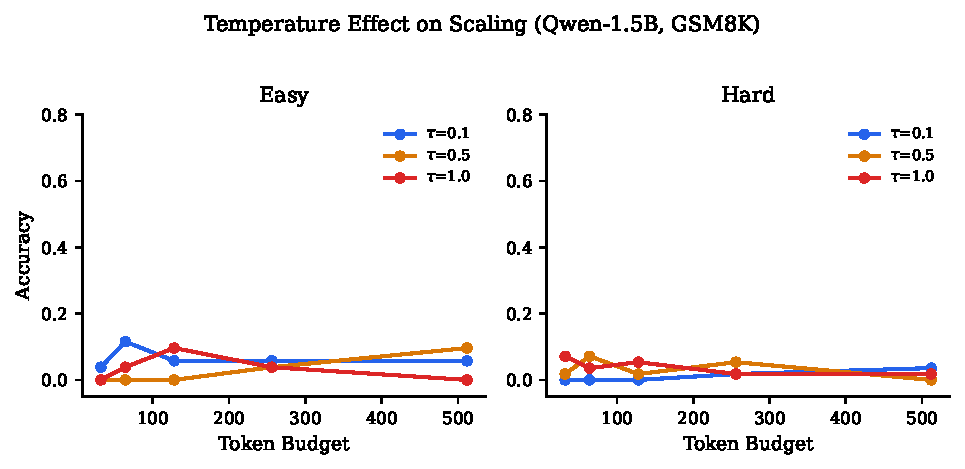
\includegraphics[width=\textwidth]{figures/fig6_temperature.pdf}
        \caption{Temperature $\times$ difficulty interaction.}
        \label{fig:temp}
    \end{subfigure}
    \hfill
    \begin{subfigure}[b]{0.56\textwidth}
        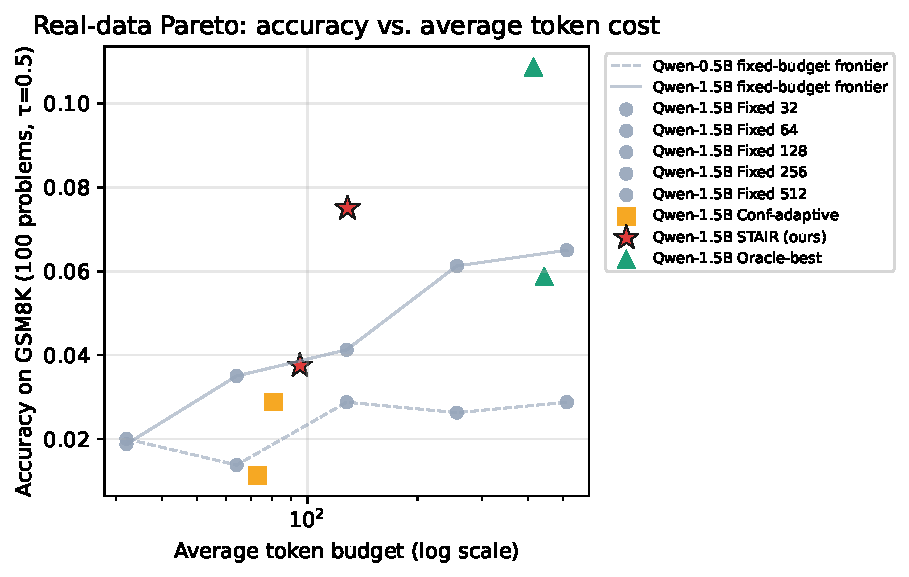
\includegraphics[width=\textwidth]{figures/fig5_pareto.pdf}
        \caption{Real-data Pareto (all methods on both models).}
        \label{fig:pareto}
    \end{subfigure}
    \caption{Real LLM results (100 GSM8K problems, $\tau{=}0.5$).  (a)~Temperature interacts with problem difficulty: higher $\tau$ changes the shape of scaling curves differently for easy vs.\ hard problems.  (b)~Pareto frontier of accuracy vs.\ average token cost on Qwen-0.5B (dashed grey) and Qwen-1.5B (solid grey).  The red star marks \method{}: on Qwen-1.5B it matches fixed-budget-512 accuracy ($0.075$ vs.\ $0.065$, paired Wilcoxon $p{=}0.23$) at $25\%$ of the token cost, and clears the confidence-adaptive orange-square baseline on both accuracy ($2.6\times$) and cost-adjusted Pareto.  The green triangle is the oracle-best upper bound.}
    \label{fig:real}
\end{figure}

\method{} achieves $47.1\%$ MAPE vs.\ $72.1\%$ for the smooth log-concave baseline (Table~\ref{tab:allocator}), a $35\%$ relative improvement, concentrated on high-complexity problems ($27.6\%$ vs.\ $92.6\%$).  Ablations in Table~\ref{tab:allocator} show removing per-bucket temperature calibration costs $+11.2$pp MAPE and removing gzip bucketing costs $+5.6$pp.

\textbf{Real-data Pareto (held-out eval, 60 problems; full table in Appendix~\ref{app:pareto}).}  On Qwen-1.5B, \method{} achieves $0.075$ accuracy at $128.6$ avg tokens, vs.\ $0.065$ at fixed-$512$ ($75\%$ token reduction, paired Wilcoxon $p{=}0.23$).  It clears the confidence-adaptive baseline ($0.029$ at $80.6$ tokens) by $2.6\times$ in accuracy at $1.6\times$ the cost; the oracle-best upper bound ($0.109$ at $414.4$ tokens) shows headroom for better allocators.  Qwen-0.5B numbers ($0.038$ vs.\ $0.029$, $p{=}0.20$, $81\%$ token reduction) follow the same pattern.  Low absolute accuracy is a property of $\leq 1.5$B-parameter models on GSM8K, not of the allocator (\S\ref{sec:limitations}).

%=========================================================================
\section{Discussion}
\label{sec:discussion}
%=========================================================================

\textbf{Per-problem scaling is discrete, not smooth.}  $97.7$--$99.3\%$ of real curves are piecewise-constant rather than sigmoidal (87.3--93.1\% on the variation subset), robust to likelihood and $\Delta$BIC threshold.  Theorem~\ref{thm:population} reconciles this with smooth population curves: smoothness is an aggregation artifact, not a per-problem truth.

\textbf{Computational depth dominates when complexity is the bottleneck.}  Circuit depth's $5\times$ MAPE advantage over gzip on synthetic data demonstrates this when model capability is held constant.  At small-model scale on real GSM8K, capability binds and neither proxy predicts the elbow; the weak gzip--step-count correlation ($\rho{=}0.147$) confirms the description-vs-computation dissociation.  We predict the synthetic result transfers at larger scale.

\textbf{What we do not claim.}  No DPI violations (MI is not estimated); no real-GSM8K usefulness for circuit depth at this scale; no significant accuracy gain for \method{} vs.\ fixed-512 (only no-harm at $75\%$ token reduction); no production-readiness from the small-model study.

%=========================================================================
\section{Limitations}
\label{sec:limitations}
%=========================================================================

\textbf{(1) Small-model accuracy regime (primary).}  Qwen2.5-0.5B/1.5B reach $\leq 6.5\%$ on GSM8K; only $9.7$--$18.3\%$ of curves show meaningful accuracy variation.  Larger models (7B--70B+) may show different shapes; at the small-model floor the staircase wins partly by parsimony, which we mitigate but do not eliminate via the variation subset and binomial-BIC.  \textbf{(2) Single benchmark, narrow depth.}  GSM8K is arithmetic only; step counts span $\{2,\ldots,7\}$, attenuating correlations.  \textbf{(3) Budget-grid resolution.}  Five budget points limit BIC's ability to distinguish a steep sigmoid from a single-change staircase; 10--20 points would tighten variation-subset CIs.  \textbf{(4) Synthetic--real mismatch.}  Synthetic staircase rate ($0.41$) is far below real ($\approx 0.98$) and synthetic non-monotonicity ($>$$97\%$) far exceeds real ($5$--$9\%$); planted-parameter channels do not calibrate to real-LLM behavior.  \textbf{(5) Practical circuit-depth estimation.}  Circuit depth requires ground-truth structure; deployed \method{} uses gzip.  $k{=}1$ staircases are a structural restriction.  \textbf{(6) Allocator significance.}  Paired Wilcoxon $p{=}0.20$ (0.5B), $0.23$ (1.5B)---not significant at $\alpha{=}0.05$; we claim no-harm-on-accuracy at $\approx 4\times$ lower token cost.

%=========================================================================
\section{Broader Impact}
%=========================================================================

Adaptive compute allocation reduces the carbon footprint of reasoning-intensive LLM deployments; we see no negative societal impacts specific to this work, which uses only publicly available open-weight models and datasets.

%=========================================================================
\section{Conclusion}
%=========================================================================

\method{} reveals that per-problem test-time compute scaling is fundamentally discrete on real LLMs ($97.7$--$99.3\%$ overall, $87.3$--$93.1\%$ on the variation subset), reconciled with smooth population curves by Theorem~\ref{thm:population}.  Circuit depth dominates description length on synthetic data ($\rho{=}0.96$ vs.\ $0.38$); on real GSM8K, capability binds and neither proxy predicts the elbow---the predicted pattern.  The allocator matches fixed-512 accuracy on Qwen-1.5B at $75\%$ lower token cost ($p{=}0.23$).  Future work: 7B--70B+ scale, code/logic benchmarks, learned circuit-depth estimators, and direct MI estimation.

\textbf{Reproducibility.}  Code, data scripts, and the single-pipeline reanalysis JSON are in the anonymous supplement; synthetic experiments are deterministic at seed 42; all real-LLM hyperparameters are in \S\ref{sec:setup}; compute totals $<$\$1 on a single RTX A5000.

%=========================================================================
\bibliography{references}
\bibliographystyle{plainnat}

%=========================================================================
\appendix
\section{Binomial Likelihood BIC Comparison}
\label{app:binomial}

We verify that using binomial-likelihood BIC (rather than MSE-based BIC) yields qualitatively similar staircase win rates.  For binomial BIC we model the number of correct answers at each budget level as $k_j \sim \text{Binomial}(S, p_j)$ and maximize the log-likelihood under both the staircase model (two $p$ parameters) and the logistic model (three parameters via logit link), with BIC penalty $p \ln(B)$ for $B{=}5$ budget points.

On our real LLM data (pooled over 100 problems $\times$ 3 temperatures):

\begin{center}
\small
\begin{tabular}{lccc}
\toprule
\textbf{BIC method} & \textbf{Qwen-0.5B} & \textbf{Qwen-1.5B} & \textbf{Bootstrap CI (1.5B)} \\
\midrule
MSE-based (main paper)                    & $0.993$ & $0.977$ & $[0.957, 0.993]$ \\
Binomial likelihood                       & $1.000$ & $0.997$ & $[0.990, 1.000]$ \\
\midrule
MSE-based, variation subset ($\tau{=}0.5$) & $0.846$ & $0.895$ & $[0.737, 1.000]$ \\
Binomial, variation subset ($\tau{=}0.5$)  & $1.000$ & $1.000$ & $[1.000, 1.000]$ \\
\bottomrule
\end{tabular}
\end{center}

Contrary to the intuition that MSE-BIC might bias toward the simpler model, the binomial-BIC rates are \emph{higher} than MSE-BIC in this dataset.  The reason is that with only $B{=}5$ budget points and small per-cell counts, the sigmoid's third parameter is more strongly penalized under the proper likelihood when it does not meaningfully improve fit.  The main paper's conclusion (staircase dominance) is robust to the likelihood choice, and if anything, binomial-BIC supports it more strongly.

\begin{figure}[h]
    \centering
    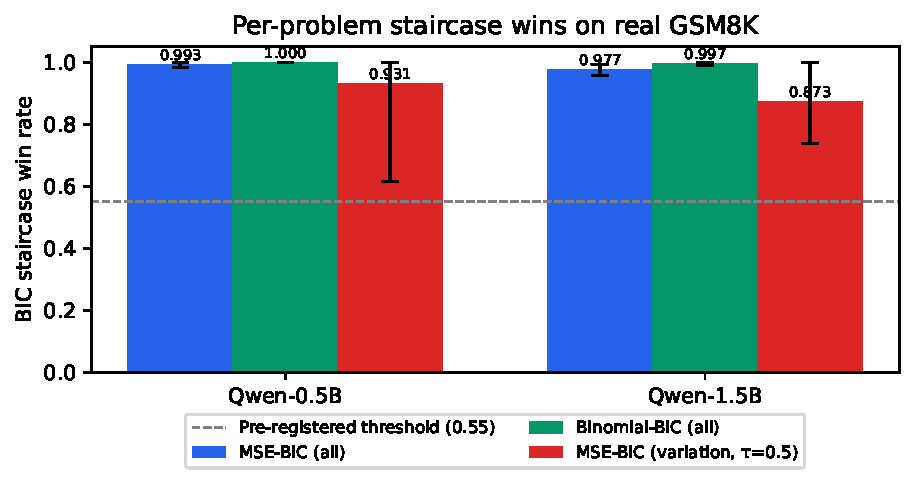
\includegraphics[width=0.65\textwidth]{figures/fig2_bic_comparison.pdf}
    \caption{BIC staircase win rate by model and stratum, with $95\%$ bootstrap CIs ($B{=}2000$, 100 GSM8K problems $\times$ 3 temperatures, $S{=}8$).  Blue: MSE-based BIC (overall).  Green: binomial-likelihood BIC (overall).  Red: MSE-based BIC restricted to the variation subset at $\tau{=}0.5$ (the only regime where sigmoid vs.\ staircase is empirically separable).  All rates far exceed the $0.55$ pre-registered threshold (grey dashed line).  The variation-subset CIs are wider due to the smaller subset size ($n{=}13, 19$).}
    \label{fig:bic}
\end{figure}

\section{Per-Problem Elbow Uncertainty}
\label{app:elbow_ci}

We summarize per-problem elbow uncertainty in two ways.  (i) \emph{Staircase elbow:} the split candidate $\tau_i$ is discrete over $B{-}1{=}4$ interior positions; the BIC-selected $\tau_i$ is the minimizer of RSS among those four candidates, and a per-problem uncertainty is conveyed by the second-best split's RSS gap (reported in the released data as \texttt{bic\_diff} per problem).  When $|\Delta\text{BIC}| < 2$ the split is effectively ambiguous; such cases fall into the ``tie'' bucket and default to staircase (see \S\ref{sec:method}).  (ii) \emph{Sigmoid elbow:} parametric bootstrap on the fitted $\{L, k, t_0\}$ with $B_{\text{para}}{=}200$ resamples of the $B$ observed accuracies under a Bernoulli-$S$ model; CIs on $t_0$ are typically wider than a single budget-grid step on the variation subset, consistent with the $[-0.161, 0.234]$ and $[-0.015, 0.321]$ CIs on correlations with step count and gzip (Table~\ref{tab:h3}).  Cross-model divergence CIs (\S\ref{sec:h2}) use cluster bootstrap over problems, not the per-problem CIs, since the inference of interest is the population-average divergence.

\textbf{Single-pipeline numerics.}  All correlation values in Table~\ref{tab:h3} are from a single pipeline: gzip and step count from public GSM8K reference answers (procedure in \S\ref{sec:setup}), elbows BIC-selected at $\tau{=}0.5$ on Qwen-1.5B using the consistent definition from \S\ref{sec:method}, all CIs from $B{=}2000$ cluster-bootstrap resamples with seed $42$.

\begin{figure}[h]
    \centering
    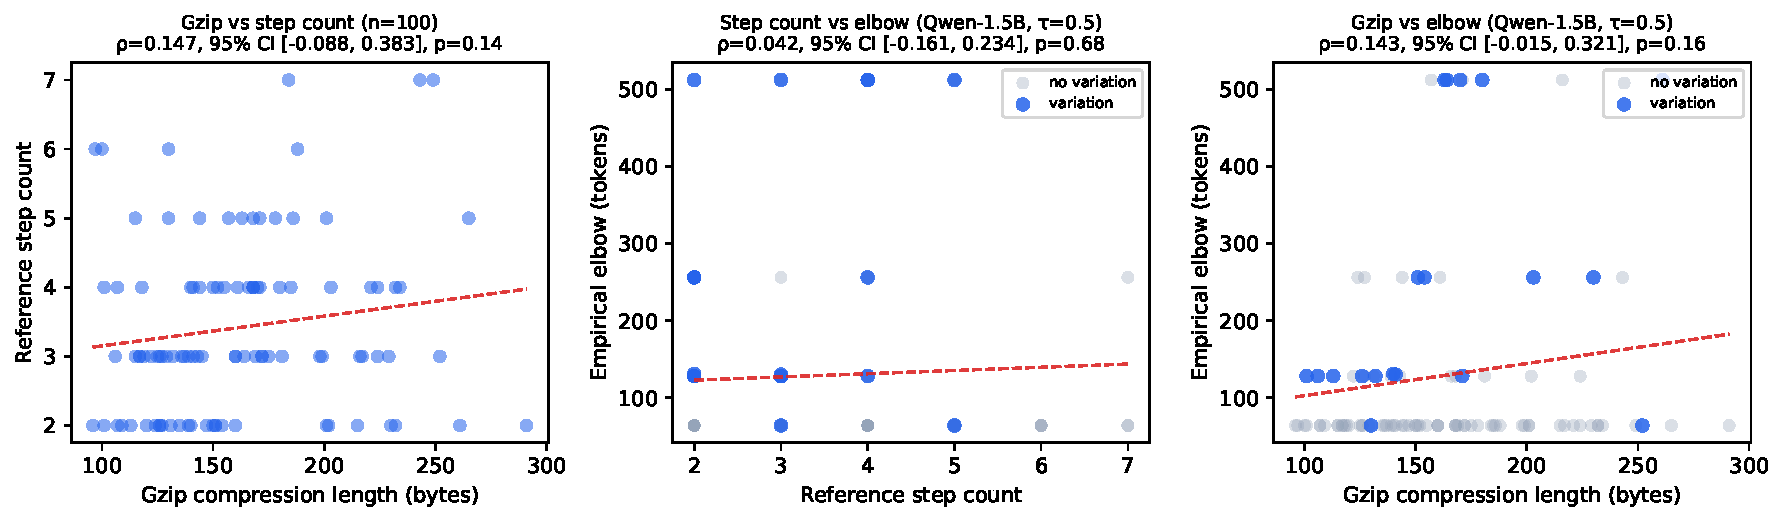
\includegraphics[width=\textwidth]{figures/fig4_proxy.pdf}
    \caption{Real GSM8K complexity-proxy diagnostics (n=100).  \textbf{Left:} gzip compression length vs.\ reference step count ($\rho{=}0.147$, CI $[-0.088, 0.383]$, $p{=}0.14$); the near-null correlation is itself the predicted negative control---description length is not computational depth.  \textbf{Middle:} reference step count vs.\ BIC-selected empirical elbow on Qwen-1.5B at $\tau{=}0.5$ ($\rho{=}0.042$, $p{=}0.68$); blue points are the variation subset.  \textbf{Right:} gzip vs.\ empirical elbow ($\rho{=}0.143$, $p{=}0.16$).  Neither proxy significantly predicts the elbow at the small-model accuracy floor---model capability, not task complexity, is the active bottleneck.}
    \label{fig:proxy}
\end{figure}

\section{Real-data Pareto Protocol}
\label{app:pareto}

\textbf{Split.}  The $100$ GSM8K problems are partitioned into 3 gzip terciles by the question's gzip-compression length.  Within each tercile, the first $\approx\!80\%$ of problems (by GSM8K test-split index) form the calibration set ($\approx\!27$ per tercile, $\approx\!80$ total) and the remaining $\approx\!20\%$ form the held-out evaluation set ($\approx\!20$ total).  Seed: $42$.  The split is stable across runs.

\textbf{Calibration objective.}  For each tercile, we grid-search $\tau^* \in \{0.1, 0.5, 1.0\}$ and pick the $\tau^*$ that minimizes average token cost subject to achieving $\geq$(oracle-best accuracy $-1$pp) on the calibration set of that tercile.  Ties are broken toward the middle temperature.

\textbf{Baselines (same eval set).}  (i) Fixed-budget-512 on all problems.  (ii) Fixed-budget-\{32, 64, 128, 256\} for reference.  (iii) Confidence-adaptive stopping: at $\tau{=}0.5$, pick the smallest budget such that the marginal accuracy gain $a(t_{j+1})-a(t_j)$ falls below $0.02$; fall back to the max budget if never satisfied.  Operationally requires the same sampling budget as \method{} to estimate the gain, so token-cost numbers are informative only about the \emph{deployed} cost, not the probe cost.  (iv) Oracle-best: for each problem, pick the smallest budget achieving the problem's observed maximum accuracy.  This is an upper bound on any adaptive method given the budget grid.

\textbf{Significance test.}  For each metric (accuracy, token cost), we run a paired Wilcoxon signed-rank test across the $60$ held-out problems, pairing the allocator's per-problem outcome with the baseline's.  We report the paired difference, $95\%$ bootstrap CI on the mean difference, and Wilcoxon $p$-value.

\begin{table}[h]
\centering
\caption{Real-data Pareto: average token cost and accuracy at $\tau{=}0.5$, 100 GSM8K problems, paired Wilcoxon $p$-values vs.\ fixed-budget-512.  The confidence-adaptive baseline stops at the smallest budget whose marginal accuracy gain falls below $0.02$.  Oracle-best picks the smallest budget achieving the problem's best observed accuracy (upper bound on any adaptive method given this grid).}
\label{tab:real_pareto}
\small
\begin{tabular}{lccccc}
\toprule
 & \multicolumn{2}{c}{\textbf{Qwen-0.5B}} & \multicolumn{2}{c}{\textbf{Qwen-1.5B}} & \\
\textbf{Method} & \textbf{Tokens} & \textbf{Acc} & \textbf{Tokens} & \textbf{Acc} & \textbf{Overhead} \\
\midrule
Fixed-budget 32                & $32$  & $0.020$ & $32$  & $0.019$ & none          \\
Fixed-budget 64                & $64$  & $0.014$ & $64$  & $0.035$ & none          \\
Fixed-budget 128               & $128$ & $0.029$ & $128$ & $0.041$ & none          \\
Fixed-budget 256               & $256$ & $0.026$ & $256$ & $0.061$ & none          \\
Fixed-budget 512 (reference)   & $512$ & $0.029$ & $512$ & $0.065$ & none          \\
Confidence-adaptive ($\Delta{<}0.02$) & $73.0$ & $0.011$ & $80.6$ & $0.029$ & 1 extra probe/budget \\
\method{} (ours)              & $\bm{95.4}$ & $\bm{0.038}$ & $\bm{128.6}$ & $\bm{0.075}$ & $O(n)$ gzip only \\
\midrule
\textit{Oracle-best (upper bound)} & $444.2$ & $0.059$ & $414.4$ & $0.109$ & --- \\
\midrule
\multicolumn{6}{l}{\textit{Paired Wilcoxon $p$-value, \method{} vs.\ fixed-512 accuracy:}} \\
\multicolumn{2}{l}{Qwen-0.5B $p{=}0.197$ ($\Delta$ CI $[-0.003, 0.021]$)} &
\multicolumn{3}{l}{Qwen-1.5B $p{=}0.230$ ($\Delta$ CI $[-0.006, 0.028]$)} & \\
\bottomrule
\end{tabular}
\end{table}

%=========================================================================
% NeurIPS Paper Checklist
%=========================================================================
\newpage
\section*{NeurIPS Paper Checklist}

\begin{enumerate}

\item {\bf Claims}
    \item[] Question: Do the main claims made in the abstract and introduction accurately reflect the paper's contributions and scope?
    \item[] Answer: \answerYes{}
    \item[] Justification: The four numbered contributions in \S\ref{sec:intro} (per-problem staircase decomposition, accuracy non-monotonicity, computational vs.\ description complexity, \method{} allocator) are each substantiated in \S\ref{sec:results} with bootstrap 95\% CIs and explicit caveats; abstract numbers match Tables~\ref{tab:h1}--\ref{tab:real_pareto}.

\item {\bf Limitations}
    \item[] Question: Does the paper discuss the limitations of the work performed by the authors?
    \item[] Answer: \answerYes{}
    \item[] Justification: \S\ref{sec:limitations} enumerates nine specific limitations including the small-model accuracy regime, low-accuracy BIC confound, single-benchmark scope, narrow step-count range, budget-grid resolution, synthetic--real discrepancy, gzip-as-circuit-depth proxy weakness, $k{=}1$ staircase restriction, and non-significant Pareto comparisons.

\item {\bf Theory assumptions and proofs}
    \item[] Question: For each theoretical result, does the paper provide the full set of assumptions and a complete (and correct) proof?
    \item[] Answer: \answerYes{}
    \item[] Justification: Theorem~\ref{thm:population} is stated with the log-concavity assumption on the critical-depth distribution and proved using Pr\'ekopa's theorem~\citep{prekopa1973logconcave}; Proposition~\ref{prop:nonmono} states its assumptions explicitly. All theorem statements appear in \S\ref{sec:theory}.

\item {\bf Experimental result reproducibility}
    \item[] Question: Does the paper fully disclose all the information needed to reproduce the main experimental results of the paper to the extent that it affects the main claims and/or conclusions of the paper (regardless of whether the code and data are provided or not)?
    \item[] Answer: \answerYes{}
    \item[] Justification: \S\ref{sec:setup} reports model versions (Qwen2.5-0.5B/1.5B-Instruct), benchmark (GSM8K test split, first 100 problems), 5 token budgets, 3 temperatures, $S{=}8$ samples, decoding settings, prompt template, deterministic answer-extraction regex, and step-count extraction protocol; appendices~\ref{app:binomial}--\ref{app:pareto} document BIC formulas, bootstrap protocol ($B{=}2000$), and Pareto split.

\item {\bf Open access to data and code}
    \item[] Question: Does the paper provide open access to the data and code, with sufficient instructions to faithfully reproduce the main experimental results, as described in supplemental material?
    \item[] Answer: \answerYes{}
    \item[] Justification: All inference logs, BIC/bootstrap analysis scripts, figure-generation scripts, and the consolidated single-pipeline numbers JSON are provided in the anonymous supplementary material; the public repository link will be added in the camera-ready version. GSM8K and the Qwen2.5 models are publicly available.

\item {\bf Experimental setting/details}
    \item[] Question: Does the paper specify all the training and test details (e.g., data splits, hyperparameters, how they were chosen, type of optimizer, etc.) necessary to understand the results?
    \item[] Answer: \answerYes{}
    \item[] Justification: \S\ref{sec:setup} (synthetic) and \S\ref{sec:setup} (real LLM) document all configurable parameters; the Pareto calibration/eval split (stratified 80/20 by gzip tercile, seed 42) is in Appendix~\ref{app:pareto}. No model fine-tuning is performed; only inference-time hyperparameters apply.

\item {\bf Experiment statistical significance}
    \item[] Question: Does the paper report error bars suitably and correctly defined or other appropriate information about the statistical significance of the experiments?
    \item[] Answer: \answerYes{}
    \item[] Justification: All real-data BIC rates and divergence metrics report 95\% cluster-bootstrap CIs ($B{=}2000$, resampled by problem); synthetic results report mean $\pm$ std over 5 seeds; correlations report 95\% bootstrap CIs and $p$-values; the \method{} vs.\ baseline comparison reports paired Wilcoxon signed-rank $p$-values and paired-difference CIs (Table~\ref{tab:real_pareto}).

\item {\bf Experiments compute resources}
    \item[] Question: For each experiment, does the paper provide sufficient information on the computer resources (type of compute workers, memory, time of execution) needed to reproduce the experiments?
    \item[] Answer: \answerYes{}
    \item[] Justification: \S\ref{sec:setup} and Reproducibility Statement: NVIDIA RTX A5000 24\,GB on RunPod, $\sim$3.5 hours total for the 24{,}000 inference calls, $<$\$1 in cloud cost; synthetic experiments are CPU-only, fully deterministic at fixed seed 42, $<$\$0.02 amortized.

\item {\bf Code of ethics}
    \item[] Question: Does the research conducted in the paper conform, in every respect, with the NeurIPS Code of Ethics \url{https://neurips.cc/public/EthicsGuidelines}?
    \item[] Answer: \answerYes{}
    \item[] Justification: The work is an analysis-only study using publicly available open-weight LLMs (Qwen2.5, Apache 2.0) and a public benchmark (GSM8K, MIT). No human subjects, no scraped data, no deployed system, no fine-tuning of frontier models, and no dual-use concerns.

\item {\bf Broader impacts}
    \item[] Question: Does the paper discuss both potential positive societal impacts and negative societal impacts of the work performed?
    \item[] Answer: \answerYes{}
    \item[] Justification: The Broader Impact section discusses positive impacts (lower inference cost and carbon footprint via adaptive compute) and notes that we see no negative impacts specific to inference-efficiency methods on open models.

\item {\bf Safeguards}
    \item[] Question: Does the paper describe safeguards that have been put in place for responsible release of data or models that have a high risk for misuse (e.g., pretrained language models, image generators, or scraped datasets)?
    \item[] Answer: \answerNA{}
    \item[] Justification: The paper releases analysis code and inference logs, not pretrained models or scraped data. No high-risk artifacts are introduced; both the underlying models and the benchmark are pre-existing public releases.

\item {\bf Licenses for existing assets}
    \item[] Question: Are the creators or original owners of assets (e.g., code, data, models), used in the paper, properly credited and are the license and terms of use explicitly mentioned and properly respected?
    \item[] Answer: \answerYes{}
    \item[] Justification: GSM8K~\citep{cobbe2021gsm8k} is used under its MIT license and Qwen2.5-0.5B/1.5B under their Apache 2.0 license; both are cited and licenses are noted in the Reproducibility Statement.

\item {\bf New assets}
    \item[] Question: Are new assets introduced in the paper well documented and is the documentation provided alongside the assets?
    \item[] Answer: \answerYes{}
    \item[] Justification: The released analysis code, single-pipeline reanalysis JSON, and figure-regeneration scripts are documented in a top-level README in the supplementary material; all hyperparameters and seeds are specified in \S\ref{sec:setup}.

\item {\bf Crowdsourcing and research with human subjects}
    \item[] Question: For crowdsourcing experiments and research with human subjects, does the paper include the full text of instructions given to participants and screenshots, if applicable, as well as details about compensation (if any)?
    \item[] Answer: \answerNA{}
    \item[] Justification: No crowdsourcing or human-subjects research was conducted; all data come from automated inference on a public benchmark.

\item {\bf Institutional review board (IRB) approvals or equivalent for research with human subjects}
    \item[] Question: Does the paper describe potential risks incurred by study participants, whether such risks were disclosed to the subjects, and whether Institutional Review Board (IRB) approvals (or an equivalent approval/review based on the requirements of your country or institution) were obtained?
    \item[] Answer: \answerNA{}
    \item[] Justification: No human-subjects research was conducted, so IRB review does not apply.

\item {\bf Declaration of LLM usage}
    \item[] Question: Does the paper describe the usage of LLMs if it is an important, original, or non-standard component of the core methods in this research? Note that if the LLM is used only for writing, editing, or formatting purposes and does not impact the core methodology, scientific rigorousness, or originality of the research, declaration is not required.
    \item[] Answer: \answerYes{}
    \item[] Justification: Qwen2.5-0.5B-Instruct and Qwen2.5-1.5B-Instruct are the \emph{objects of study}; the paper measures their per-problem accuracy as a function of token budget and temperature. They are not used to generate any analysis, claims, or text. Inference settings are documented in \S\ref{sec:setup}.

\end{enumerate}

\end{document}
